\documentclass[12pt,letterpaper,oneside]{article}

\usepackage[utf8]{inputenc}

% Paquete con configuraciones necesarias para cambiar el margen de las páginas
\usepackage[left=1.5cm, right=1.5cm, top=2.5cm, bottom=2.5cm]{geometry}
% - - - - - - - - - - - - - - - - - - - - - - - - - - - - - - - - - - - - - -

% Paquete necesario para incluir una imagen en el documento
\usepackage{graphicx}

\usepackage{amsmath}
% - - - - - - - - - - - - - - - - - - - - - - - - - - - - - - - - - - - - - -

%Paquete para utilizar múltiples columnas
\usepackage{multicol}
\setlength{\columnsep}{1cm}

% Utilizado para agregar label a los componentes que no la pueden llevar
\usepackage{caption}
\usepackage{subcaption}

%Paquete utilizado para realizar el spanning de celdas en una tabla
\usepackage{multirow}

\title{Listas y Tablas}
\author{Emilio-Ernesto Hernández-Huerfano}

\begin{document}

\maketitle

\section{Listas}

\noindent Las listas son componentes sencillos en \LaTeX, y existen de tipo \textbf{ordenada} (\ref{prop:orderedlist}.\ref{itm:important}) y \textbf{no-ordenada}:

\begin{multicols}{3}

\begin{itemize} \label{prop:unorderedlist}
	\item Elemento de la lista 1
	\item[-] cdf
	\item Elemento de la lista 2
	\item Elemento de la lista 3
\end{itemize}

\columnbreak

\begin{enumerate} \label{prop:orderedlist}
	\item ...
	\begin{enumerate} \label{prop:orderedlist}
	\item Elemento de la lista
	\item\label{itm:important} Elemento de la lista
	\item Elemento de la lista
	\end{enumerate}
	\item\label{itm:important} Elemento de la lista
	\item Elemento de la lista
\end{enumerate}

\columnbreak

\begin{enumerate} \label{prop:orderedlist}
	\item Elemento de la lista
	\item\label{itm:important} Elemento de la lista
	\item Elemento de la lista
\end{enumerate}

\end{multicols}

Efectivamente también pueden combinarse... that's your work ;)


\section*{Tablas}

\noindent Una tabla es un componente de línea separada (a diferencia de una equación que puede estar en la misma línea que el texto, como $f(x)=0$).

\begin{center}
\begin{tabular}{ l c r }
 Computación & 24 & Emilio \\ 
 Química & 10 & 35 \\ 
 Geología & 20 & 2 \\ 
\end{tabular}
\end{center}


Se utilizará el ambiente \verb|\begin{tabular}{r c c } ... \end{tabular}| para generar un componente tabla, y se le pasará como parámetro principal una cadena de caracteres que especifica el número de columnas que nuestra tabla tendrá, y la alineación de cada una de estas. Esta cadena es de la forma \verb|{ l c r }|, en donde cada letra representa una columna, y la letra \verb|'l'| significa que la orientación es a la izquierda, la \verb|'c'| significa que el texto de la columna estará centrado y la \verb|'r'| que estará alineado a la derecha.

\begin{center} %Centrando el componente (dejando ciertos espacios convenientes).
\begin{tabular}{ |c|c|c| } 
 \hline %Utilizada para generar una línea horizontal
 celda1 & celda2 & celda3 \\ 
 \hline 
 celda4 es algo larga & celda5 & celda6 \\ 
 \hline 
 celda7 & celda8 & celda9 \\ 
 \hline %Utilizada para generar una línea horizontal
\end{tabular}
\end{center}



\begin{multicols}{2}

Para agregar un header se utiliza una estructura muy similar, no hay un componente exclusivo para la cabecera de la tabla, si no que se simula con los que ya conocemos:



\begin{center}
 \begin{tabular}{||c | c | c | c||} 
 
 %Esto define que la primera fila será presentada separada del resto de las filas
 \hline
   Nombre & Apellido & Edad  \\ [0.5ex] 
 \hline \hline
 Emilio & Hernández & 26  \\ 
 \hline
 Leonardo & Álvarez & 27 \\
 \hline
 David & Saucedo & 22 \\
 \hline
\end{tabular}
\end{center}


También es posible agregar referencias a la tabla, así como un texto descriptivo de esta del tipo "pie de tabla" \ref{tab:ejemploDeReferencia}.

\begin{center}
  
  \begin{tabular}{r | l}
    material  & T [K]\\
    \hline
    Sn & 3,7 \\
    Pb & 7,2 \\
    Al & 1,2\\
  \end{tabular}
  \captionof{table}{Ejemplo de una tabla con referencia cruzada. \label{tab:ejemploDeReferencia}}
\end{center}



\end{multicols}



\begin{figure}
     \centering
     \begin{subfigure}[b]{0.3\textwidth}
         \centering
         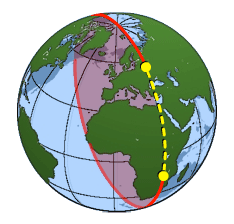
\includegraphics[width=\textwidth]{haversine.png}
         \caption{$y=x$}
         \label{fig:y equals x}
     \end{subfigure}
     \hfill
     \begin{subfigure}[b]{0.3\textwidth}
         \centering
         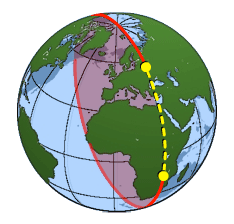
\includegraphics[width=\textwidth]{haversine.png}
         \caption{$y=3sinx$}
         \label{fig:three sin x}
     \end{subfigure}
     \hfill
     \begin{subfigure}[b]{0.3\textwidth}
         \centering
         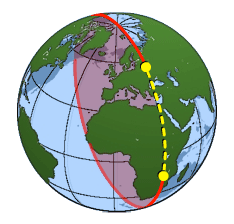
\includegraphics[width=\textwidth]{haversine.png}
         \caption{$y=5/x$}
         \label{fig:five over x}
     \end{subfigure}
        \caption{Three simple graphs}
        \label{fig:three graphs}
\end{figure}



\end{document} 